\newpage
\section{Theoretical Analysis}
\label{sec:analysis}

\subsection{Mesh Analysis}
\begin{figure}[h] \centering
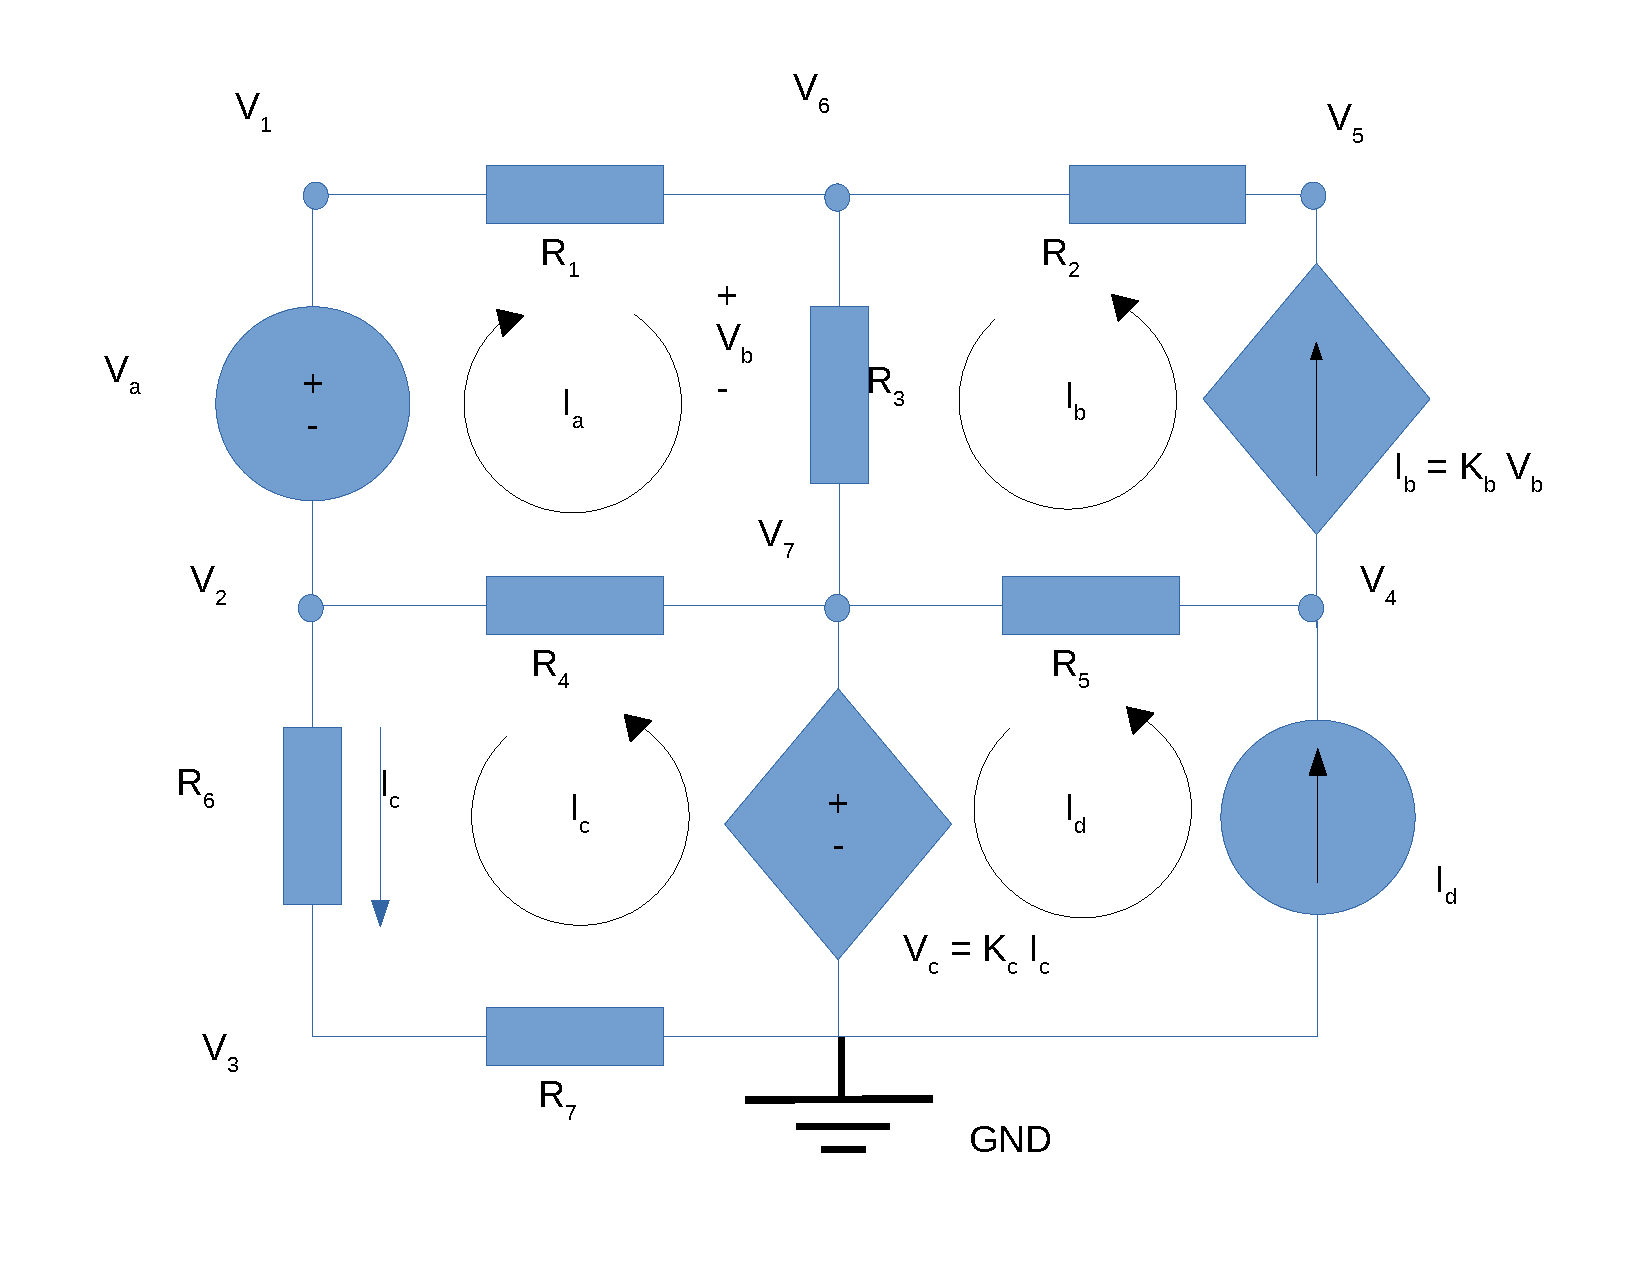
\includegraphics[width=0.8\linewidth]{rc1.pdf}
\caption{Representation of mesh currents in the circuit.}
\label{fig:meshcurrents}
\end{figure}

Figure~\ref{fig:meshcurrents} shows the mesh currents considered for the circuit analysis, with the current $I_a$ flowing clockwise and the rest of the currents ($I_b$, $I_c$ and $I_d$) flowing counter-clockwise. In the meshes containing $I_b$ and $I_d$, the currents were considered to be the same as the current sources in said meshes.

From this circuit, there can then be extracted 3 equations to figure out the value of the components necessary for the circuit analysis.

The first one, Equation~\ref{eq:meshb} , was obtained by using Ohm's Law, assuming it is known the value of the voltage and the resistence in resistor 3 and that the current flowing through it is ($I_a$ + $I_b$).
\begin{equation}
  I_{b} = K_{b}(I_{a} + I_{b})R_{3},
  \label{eq:meshb}
\end{equation}

Equation~\ref{eq:mesha}  was figured out by analysing the top left mesh, using Kirchoff's Voltage Law and Ohm's Law for the resistors. Since the current $I_a$ is flowing clockwise, the voltage in $V_a$ is negative and the currents in resistors 3 and 4 are, 
correspondingly, ($I_a$ + $I_b$) and ($I_a$ + $I_c$), as these pairs of currents are flowing the same way in said resistors.
\begin{equation}
  -V_{a} + I_{a}R_{1} + (I_{a} + I_{b})R_{3} + (I_{a} + I_{c})R_{4} = 0,
  \label{eq:mesha}
\end{equation}

Finally, from the bottom left mesh, there is Equation~\ref{eq:meshc}, in which was also used Kirchoff's Voltage Law and Ohm's Law. The voltage in $V_ac$ is negative due to the current flow.
\begin{equation}
  -K_{c}I_{c} + I_{c}R_{6} + I_{c}R_{7} + (I_{a} + I_{c})R_{4} = 0,
  \label{eq:meshc}
\end{equation}

By developing these 3 equations, the matrix below (\ref{eq:matrix}) is achieved as to simplify the calculations. This matrix was solved in Octave, getting the values of the currents $I_a$, $I_b$ and $I_c$. It was not necessary to solve for the value of the current in the bottom right mesh since it is already known (equivalent to $I_d$).
\begin{equation}
\left[ \begin{array}{ccc} -K_bR_3 & 1-K_bR_3 & 0 \\ R_1+R_3+R_4 & R_3 & R_4 \\ R_4 & 0 & R_6+R_7-K_c+R_4 \end{array} \right]
\times \left[ \begin{array}{c} I_a \\ I_b \\ I_c \end{array} \right] =
\left[ \begin{array}{c} 0 \\ V_a \\ 0 \end{array} \right]
\label{eq:matrix}
\end{equation}

The values of $I_a$, $I_b$ and $I_c$ are then, correspondingly, (2.5852e-4)V, (-2.7062e-4)V and (1.0865e-3)V. With these currents, it is possible to discover the values of the voltages in each node, using the equations~\ref{eq:node7} through~\ref{eq:node1} down below and knowing that $I_b$ = $K_b$$V_b$ and $V_c$=$K_c$$I_c$.
\begin{equation}
  V_{7} = V_{c},
  \label{eq:node7}
\end{equation}

\begin{equation}
  V_{6} = V_{7} + V_{b},
  \label{eq:node6}
\end{equation}

\begin{equation}
  V_{5} = V_{6} + R_{2}I_{b},
  \label{eq:node5}
\end{equation}

\begin{equation}
  V_{4} = V_{7} + R_{5}I_{d},
  \label{eq:node4}
\end{equation}

\begin{equation}
  V_{3} = V_{0} + R_{7}I_{c},
  \label{eq:node3}
\end{equation}

\begin{equation}
  V_{2} = V_{3} + R_{6}I_{c},
  \label{eq:node2}
\end{equation}

\begin{equation}
  V_{1} = V_{2} + V_{a},
  \label{eq:node1}
\end{equation}

The following table (\ref{table:nodesmesh}) shows the node voltages discored by replacing the variables with the known values. Notice that the values are not equal to the ones obtained by the simulation analysis or the node analysis. This is due to the fact that the mesh analysis is not as exact as the other methods; however, the results are similar enough to be relevant to this experiment.
\begin{table}[h!]
\centering
\begin{tabular}{ |c|c| } 
 \hline
 {\bf Node} & {\bf Voltage[V]} \\ 
 \hline\hline
 $V_1$ & 8.5206e00 \\ 
 \hline
 $V_2$ & 3.2785e00 \\ 
 \hline
 $V_3$ & 1.0920e00 \\ 
 \hline
 $V_4$ & 1.1956e01 \\ 
 \hline
 $V_5$ & 7.4396e00 \\ 
 \hline
 $V_6$ & 7.9946e00 \\ 
 \hline
 $V_7$ & 8.8313e00 \\ 
 \hline
\end{tabular}
\caption{Voltage values using the mesh analysis.}
\label{table:nodesmesh}
\end{table}

\subsection{Nodal Analysis}
